\section{Zielsetzung}
    Ziel des Versuches ist es, die Brennweiten verschiedener Linsen zu bestimmen, wobei verschiedene Methoden anzuwenden sind. Des Weiteren 
    sollen das Abbildungsgesetz, sowie die Linsengleichung verifiziert werden. Es wird ebenfalls die chromatische Abberation untersucht.

\section{Theorie}
\label{sec:theorie}
    Linsen bestehen im Allgemeinen aus einem Material, welches optisch dichter als die Umgebungsluft ist, das heißt einen höheren 
    Brechungsindex aufweist als der von Luft. Dabei wird zwischen Sammellinsen und Zerstreuungslinsen unterschieden. Bei Sammellinsen 
    werden wie in \autoref{fig:sammel} zu sehen parallele Strahlen im Brennpunkt gebündelt und es entsteht ein reelles Bild. Die 
    Brennweite $f$ und die Bildweite $b$ sind dabei positive Werte. Im Gegensatz dazu sind bei Zerstreuungslinsen, wie in
    \autoref{fig:zerstreu} zu sehen, die Brennweite $f$ und Bildweite $b$ negativ, sodass ein virtuelles Bild ensteht.
    Dies gilt allerdings nur für dünne Linsen. Bei dicken Linsen lässt sich die Brechung nicht mehr auf die Mittelebene der
    Linse reduzieren; stattdessen werden, wie in \autoref{fig:dick} dargestellt, zwei Hauptebenen eingeführt.
    \begin{figure}
        \centering
        \begin{subfigure}{0.48\textwidth}
            \centering
            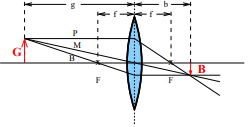
\includegraphics{content/sammel.png}
            \caption{Sammellinse.}
            \label{fig:sammel}
        \end{subfigure}
            \begin{subfigure}{0.48\textwidth}
            \centering
            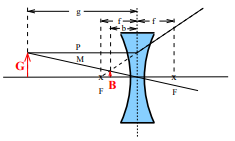
\includegraphics{content/zerstreu.png}
            \caption{Zerstreuungslinse.}
            \label{fig:zerstreu}
        \end{subfigure}
        \begin{subfigure}{0.48\textwidth}
            \centering
            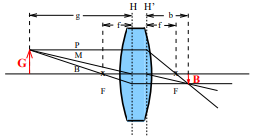
\includegraphics{content/dick.png}
            \caption{Dicke Sammellinse.}
            \label{fig:dick}
        \end{subfigure}
            \caption{Schematische Darstellung verschiedener Linsensysteme.}
            \label{fig:linsen}
        \end{figure}
    Bei der Bildkonstruktion
    sind, wie in den Abbildungen zu sehen, drei verschiedene Strahlen relevant. Erstens verläuft der sogenannte Parallelstrahl parallel 
    zur optischen Achse und wird von der Linse so gebrochen, dass er durch den Brennpunkt läuft. Zweitens läuft der Mittelpunktstrahl
    vom Objekt zum Mittelpunkt der Linse und verändert seine Richtung nicht. Drittens verläuft der Brennpunktstrahl durch den Brennpunkt
    zur Linse und wird dort so gebrochen, dass er sich danach parallel zur optischen Achse ausbreitet.

    Über die Strahlensätze lässt sich das Abbildungsgesetz
    \begin{equation}
    \label{eqn:abbildung}
        V = \frac{B}{G} = \frac{b}{g} 
    \end{equation}
    herleiten, wobei $V$ der Abbildungsmaßstab, $B$ die Bildgröße, $G$ die Gegenstandsgröße, $b$ die Bildweite und $g$ die Gegenstandsweite 
    bezeichnet. Mittels Gleichung \eqref{eqn:abbildung} lässt sich des Weiteren für dünne Linsen die Linsengleichung
    \begin{equation}
    \label{eqn:linsen}
        \frac{1}{f} = \frac{1}{b} + \frac{1}{g}
    \end{equation}
    herleiten, wobei $f$ die Brennweite ist. 

    Generell gilt die Näherung bei dünnen Linsen, dass die Brechung nur an der Mittelebene der Linse stattfindet, nur für achsennahe 
    Strahlen. Für achsenferne Strahlen können Abbildungsfehler auftreten, da diese stärker gebrochen werden. Dieser Effekt wird
    sphärische Abberation genannt und kann dafür sorgen, dass sich kein scharfes Bild erzeugen lässt, 
    da der Brennpunkt achsenferner Strahlen näher an der Linse liegt, als der von
    achsennahen Strahlen. Dies lässt sich aber zum Beispiel durch Verwendung einer Irisblende
    vermeiden, da diese die achsenfernen Strahlen ausblendet. Ein weiterer Abbildungsfehler ist die sogenannte chromatische Abberation.
    Dieser ensteht dadurch, dass der Brennpunkt von blauem Licht näher an der Linse liegt, als der Brennpunkt von rotem Licht. Das
    führt dazu, dass das blaue Licht stärker gebrochen wird als rotes Licht.

    \subsection{Methoden zur Bestimmung der Brennweite $f$} 
    In diesem Versuch werden zwei verschiedene Methoden zur Bestimmung von Brennweiten angewandt. 
    \subsubsection{Methode nach Bessel}
        \begin{figure}
            \centering
            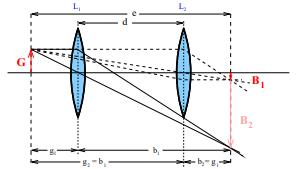
\includegraphics[width=0.48\textwidth]{content/bessel.png}
            \caption{Schematische Darstellung zur Bestimmung der Brennweite nach der Methode von Bessel.}
            \label{fig:bessel}
        \end{figure}
        Bei der Methode nach Bessel wird der Abstand $e$ zwischen einem Gegenstand und Schirm konstant gehalten (siehe \autoref{fig:bessel}).
        Dieser sollte dabei mindestens viermal so groß wie die Brennweite $f$ der Linse sein. Die zu untersuchende Linse wird zwischen dem
        Gegenstand und dem Schirm bewegt und auf die zwei Positionen eingestellt, an denen ein scharfes Bild ensteht. Zu beiden Postionen
        werden die Bildweite $b$ beziehungsweise Gegenstandsweite $g$ notiert, wobei hier eine Symmetrie vorliegt, sodass
        \begin{align*}
        b_1 &= g_2 & b_2 &= g_1
        \end{align*}
        gilt.
        Mit dem Zusammenhang $e = b_1 + g_1 = b_2 + g_2$ und $d = g_1 - b_1 = g_2 - b_2$ kann die Brennweite $f$ zu 
        \begin{equation}
        \label{eqn:bessel}
        f = \frac{e^2 -d^2}{4 \cdot e}
        \end{equation}
        bestimmen.
    \subsubsection{Methode nach Abbe}    
        Mit der Methode von Abbe lässt sich die Brennweite eines Linsensystems beziehungsweise einer dicken Linse,
        wie in \autoref{fig:abbe} zu sehen, bestimmen. Hierzu wird die Bild- beziehungsweise Gegenstandsweite $b$ und $g$ relativ zu
        den Hauptebenen $H$ und $H'$ bestimmt. Da diese jedoch nicht bekannt sind wird ein beliebiger Punkt $A$ festgelegt, zu dem
        $b'$ und $g'$ gut messbar sind. Es gelten demnach die Relationen
        \begin{align}
        \label{eqn:abbe}
        g' &= g + h = f \cdot \Bigl(1 + \frac{1}{V}  \Bigr )+ h \\
        b' &= b + h' = f \cdot (1 + V) + h'
        \end{align}
        wobei $V$ der Abbildungsmaßstab ist und $h$ und $h'$ die Lage der Hauptebenen bezeichnet.
        \begin{figure}
            \centering
            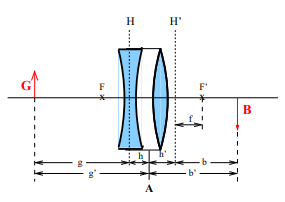
\includegraphics[width=0.48\textwidth]{content/abbe.png}
            \caption{Schematische Darstellung zur Bestimmung der Brennweite nach der Methode von Abbe.}
            \label{fig:abbe}
        \end{figure}
